\documentclass{article}
\usepackage{indentfirst}
\usepackage{tabto}
\usepackage{graphicx}
\graphicspath{ {./images/} }
\begin{document}
\section{Unified Framework}
Unified Framework in Artificial Intelligence, in a nutshell, is the general map of how inputs are processed and how outputs are derived from necessary functions. \\
\tab\tab Basically, training inputs are picked apart into concerned features through \textbf{basis functions}, and when graphed in a suitable coordinate system, they are called \textbf{coordinate vectors}. Now, we have a collection of those coordinate vectors that we can make use of later on. To use these data, we have to have an input, say, a requirement, to get the data we want. The input requirement then will also be picked apart into necessary coordinate vectors that will be used to compare it with our data set.\\
\tab \tab But there is a problem! We cannot compare incompatible things together, like comparing a stone and a human, we cannot get a definable similarity and difference. What we need to do is to make all those disparate coordinate vectors comparable. How? By projecting them into a same interface. Let's look at an example.\\
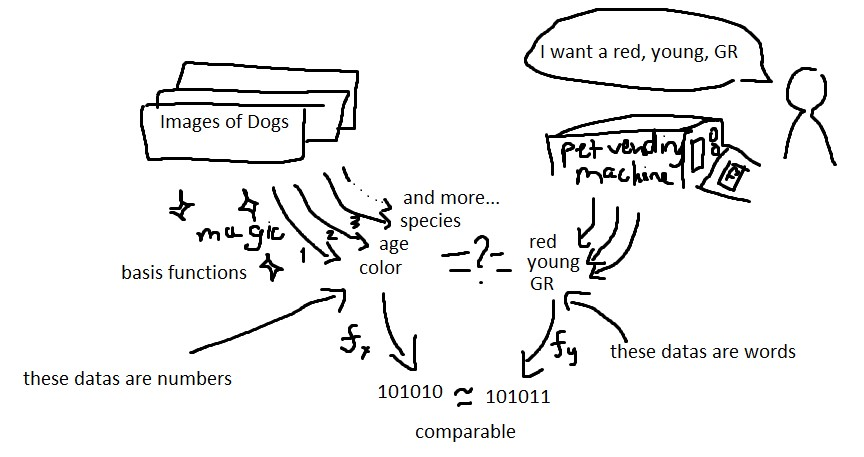
\includegraphics[scale=0.5]{img1} \\
\centerline{ \small{\textbf{Image 1.1: Unified Framwork in an AI Dog Vending Machine}}} \\\\
\tab\tab Example: You are going out to buy a dog, and when driving through a corner, you catch a glimpse of a dog vending machine. "Cool," you thought, "let's give it a try". You walk up to the machine, insert a hundred dollar bill, state your order, and voila, your brand new pet. Driving home with your new best companion, you cannot stop thinking about how that weird machine works.
\\ \tab \tab The answer is simple: The machine has already been trained of thousands and thousands of dog images, and inside its data cache is a huge collection of features, or \textbf{coordinate vectors}, that was taken from the myriads of dog images using "magic", or \textbf{basis functions}. When you speak your orders, the machine \textit{also} picks apart those words, going through a different "magic", but before actually finding your dog, the machine has to make its data collection and your order \textbf{comparable}. Going through yet another "\textit{magic}", the data collection and the order now reside in a same place, same properties. The last thing to do is to find the set of data in the dog collection that has the \textbf{minimum} error compared to your order. Magical, is it not?

\section{PCA (Principal Component Analysis)}
You are confused by my explanation about how the machine picks apart a bunch of picture. Very, in fact. "Why, and how?", enraged you walk to the vending dog machine with a sledgehammer, trying to \textit{actually} picking the machine apart to take its magic. Before you do something radical, let me assure you that you will get nothing but a bunch of chips and boards (you may even kill some puppies in it!), and there is no magic. The \textit{magic} that I have mentioned above, that can analyze important features of the pictures, is a concept called \textbf{PCA}, or \textbf{Principal Component Analysis}. \\
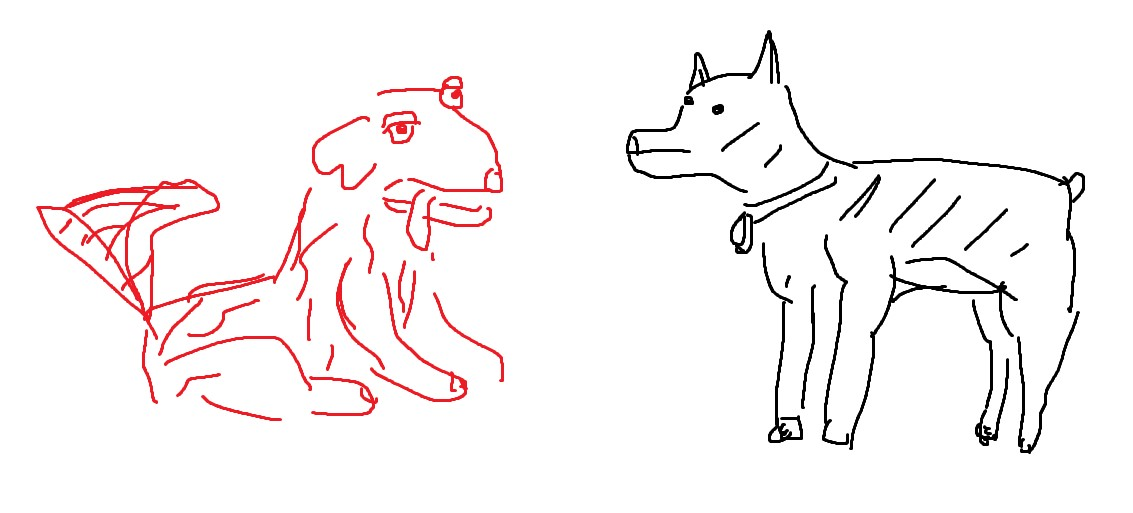
\includegraphics[scale=0.4]{img2}\\
\centerline{\small{\textbf{Image 2.1: Picture of your dog and neighbor Ray's German Shepherd}}}	\\\\
\tab\tab PCA is smart, I tell you. Look at two of these dogs. What are the differences between your dog and Ray's? The color, the breed, the posture of the dogs, it is obvious, isn't it? You readily know which is different, and what would be the features that \textbf{most} differs between the two dogs. \textit{\textbf{PCA} do the exact same thing}. \textbf {It mathematically picks out the feature that varies the most among the many objects it observed}. Train the machine to do just that a couple of a hundred more and you get yourself your own nice and well-equipped dog collection.\\\tab\tab Now drop that sledgehammer.\\\\
\tab\tab Extra information about how PCA works in theory.\\
\centerline{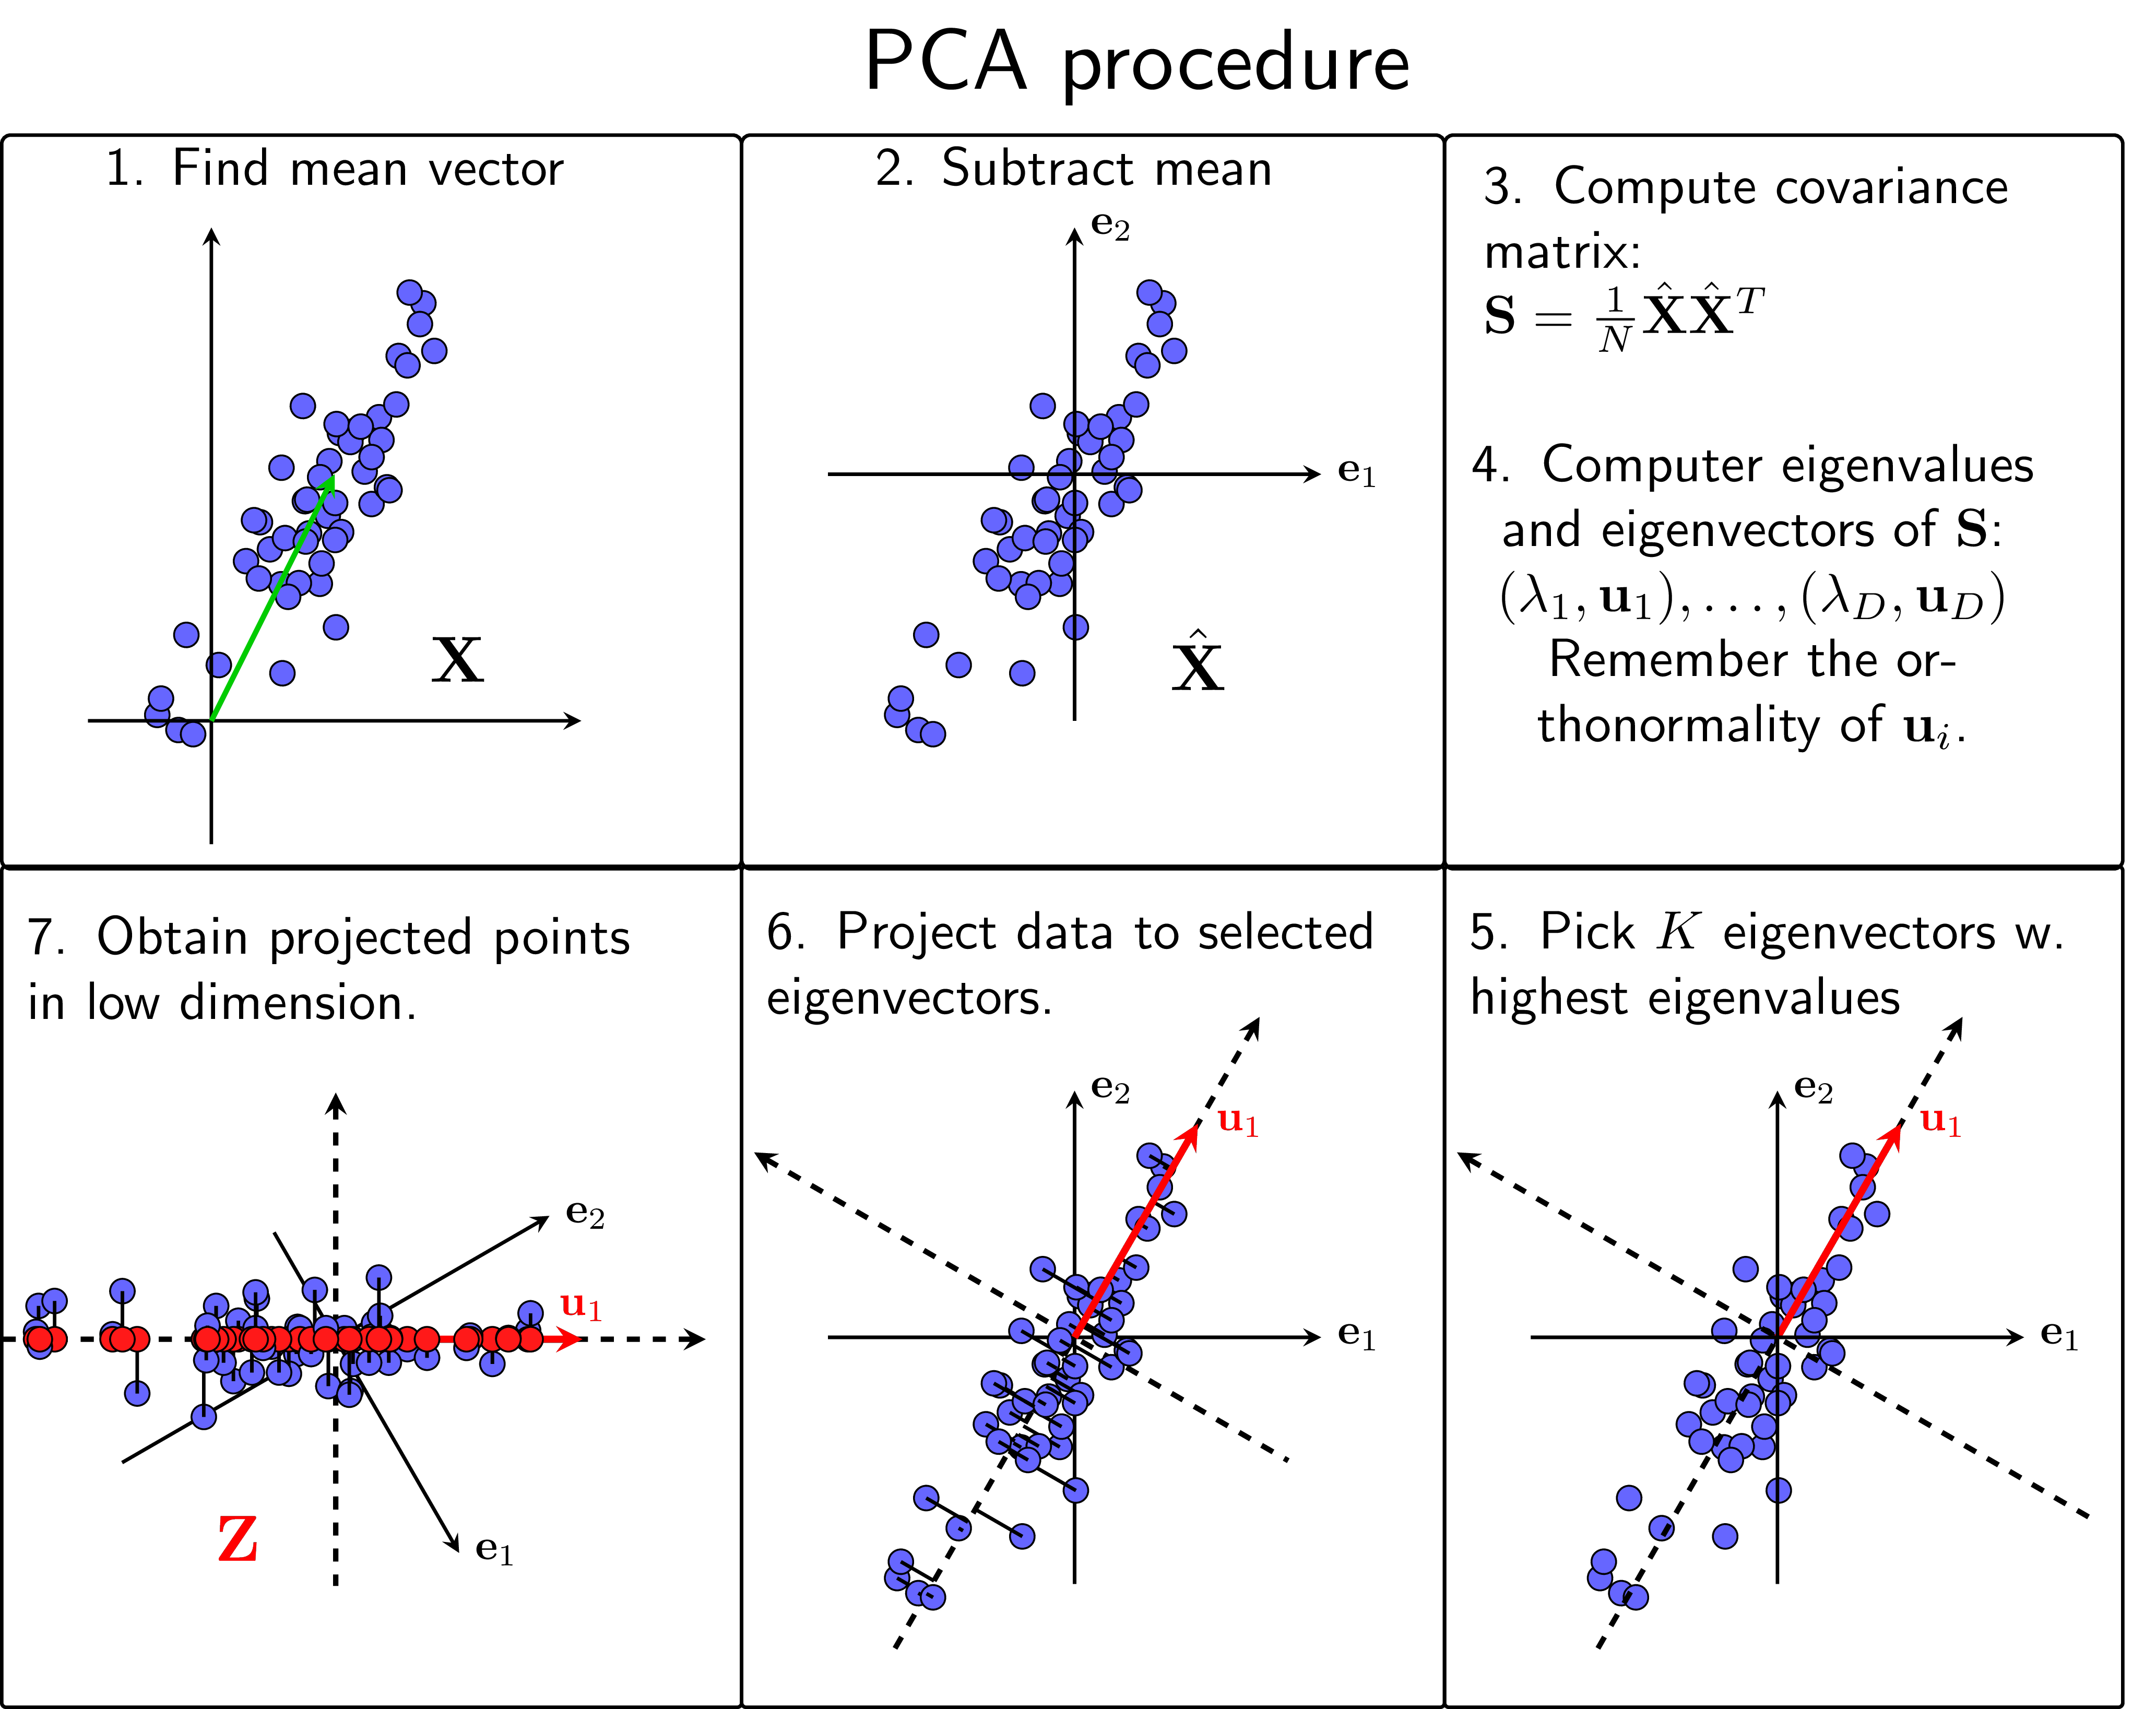
\includegraphics[scale=0.08]{img7}}
\section{Linear Regression}
	You seems satisfied that the magic is not magic at all. "All math and stuff, huh?", you murmur,"I am definitely not touching those." Suddenly, you catch the glimpse of my Fx scribble. "Wait what is that?" you ask, assuring yourself that curiosity killed the cat, not you. Well, it sure killed the cat, but it is also killing my time for sure. \\\\ \centerline{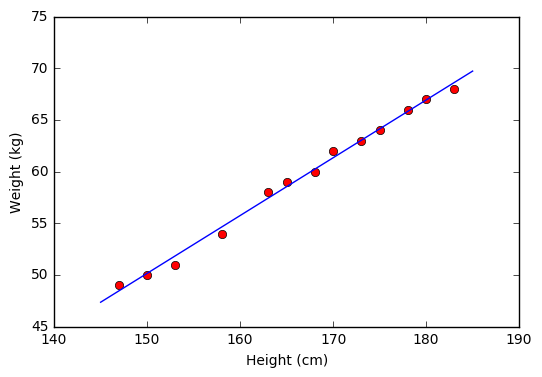
\includegraphics[scale=0.6]{img3}}\\
	\centerline{\small{\textbf{Image 3.1: Graph that represents linear regression}}}	\\\\
	\tab \tab Linear regression is the simplest way to convert your dog collection, or raw and incompatible data generally, to something that would be comparable to your input data.\\
	\tab\tab Let's take two data types from your dog collection - height and weight - and graph it.\\\\
	\centerline{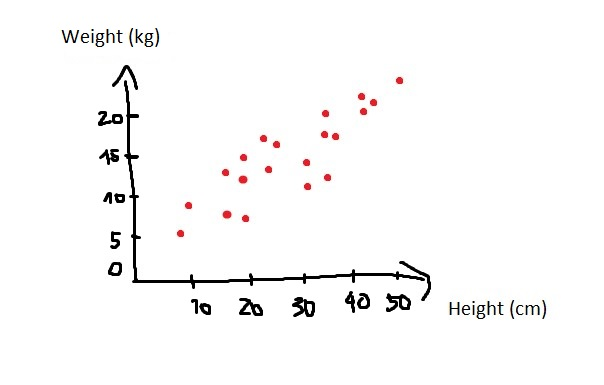
\includegraphics[scale=0.5]{img4}} \\
	\centerline{\small{\textbf{Image 3.2: Graph of dogs' height versus weight, data taken}}}	
	\centerline{\small{\textbf{ from the Dog Collection (imaginary)}}}\\\\
	\tab\tab Looking at this graph, as a human, you can obviously see there is a trend in the dog's height versus weight. Using mathematical functions, a machine can "see" this trend through the means of the \textit{line of best fit}, and from there, it can predict height or weight of a dog with a more or less acceptable errors. For example your red Golden Retriever is 40cm in height. According to this machine-generated trend line, your dog should weigh about 20kg. (graph shown in next page) \\\\
	\centerline{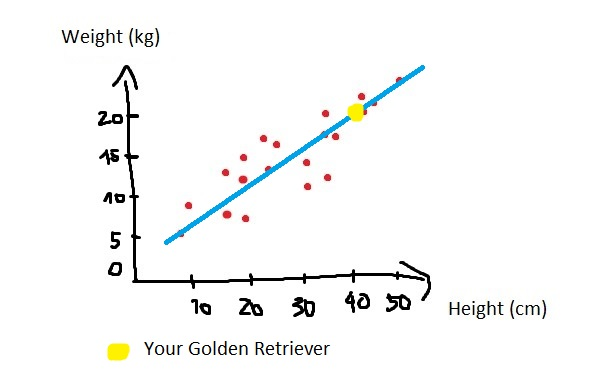
\includegraphics[scale=0.5]{img5}}	\\
	\centerline{\small{\textbf{Image 3.3: Your Golden Retriever's data on the graph}}}\\\\
	\tab\tab Though keep in mind that \textbf{Linear Regression} is not the optimal function to make your data comparable to the input. Due to the properties of the linearity, the line of best fit can be terribly wrong if there is an extreme outlier.\\
	\section{Logistic Regression}
	"Hey before you go, is there a better way to make data comparable, like, non-linear regression?" you ask. Well, there sure is.\\\\
\centerline{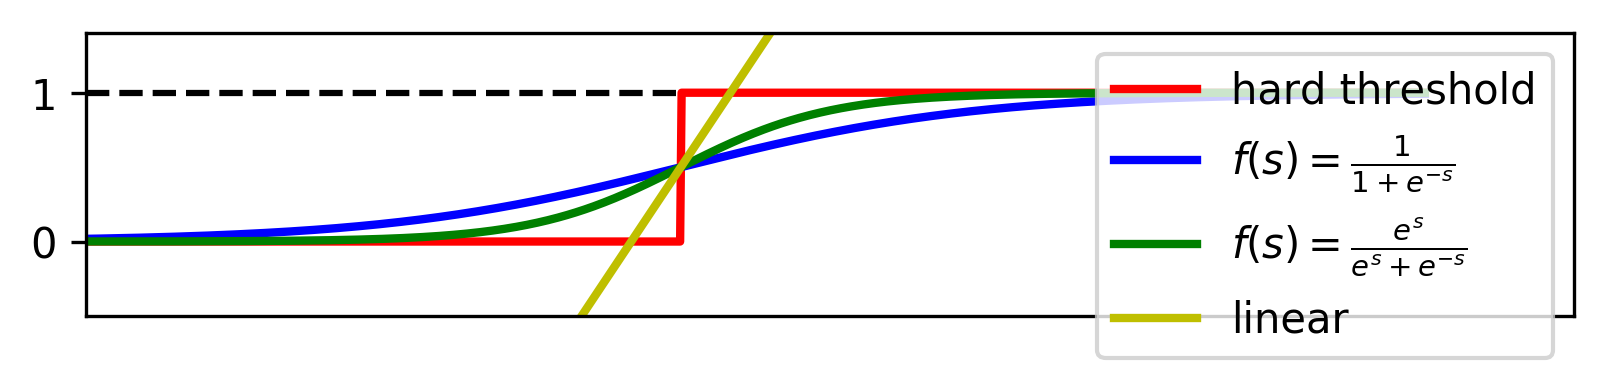
\includegraphics[scale=0.7]{img6}}\\
\centerline{\small{\textbf{ Image 4.1: Graph comparing between different regressive methods}}}\\\\ 
\tab\tab \textbf{Logistic Regression} is just another regression, fundamentally. Instead of using linear function, its line of best fit is a logistic equation, like this $$\frac{L}{1 + e^{-k(x-x_0)}}$$
\tab or more simply $$\frac{1}{1 + e^{-s}}$$\\
\tab\tab The advantage of logistic regression is that it is \textbf{much more \textit{flexible}} than linear regression, as displayed in the above graph, delivering even better accuracy.
\end{document}